\documentclass[journal]{IEEEtran}
\usepackage[a5paper, margin:10mm, onecolumn]{geometry}
\usepackage{amsmath,amssymb,amsfonts,amsthm}
\usepackage{mathtools}
\usepackage{gvv-book}
\usepackage{gvv}
\usepackage{hyperref}

\begin{document}

\title{12.683}
\author{Puni Aditya - EE25BTECH11046}
\maketitle

\textbf{Question:}

The unit normal vector to the surface $X^2 + Y^2 + Z^2 - 48 = 0$ at the point (4, 4, 4) is \rule{2cm}{0.4pt}.

\textbf{Solution:}

Let the surface be defined by the level set of a function $f\brak{\vec{x}} = 0$.
\begin{align}
    f\brak{X, Y, Z} = X^2 + Y^2 + Z^2 - 48
\end{align}
The normal vector to the surface at any point is given by the gradient of the function, $\nabla f$.
\begin{align}
    \nabla f = \myvec{\frac{\partial f}{\partial X} \\ \frac{\partial f}{\partial Y} \\ \frac{\partial f}{\partial Z}} = \myvec{2X \\ 2Y \\ 2Z} \label{eq:27}
\end{align}
Substituting 
\begin{align}
    \vec{p} = \myvec{4 \\ 4 \\ 4}
\end{align}
in \eqref{eq:27}
\begin{align}
    \vec{n} = \nabla f\brak{\vec{p}} = \myvec{2\brak{4} \\ 2\brak{4} \\ 2\brak{4}} = \myvec{8 \\ 8 \\ 8}
\end{align}
To find the unit normal vector $\hat{\vec{n}}$,
\begin{align}
    \norm{\vec{n}} &= \sqrt{8^2 + 8^2 + 8^2} = \sqrt{3 \times 64} = 8\sqrt{3}
\end{align}
\begin{align}
    \hat{\vec{n}} = \frac{\vec{n}}{\norm{\vec{n}}} = \frac{1}{8\sqrt{3}}\myvec{8 \\ 8 \\ 8} = \frac{1}{\sqrt{3}}\myvec{1 \\ 1 \\ 1}
\end{align}

\begin{figure}[h!]
	\centering
	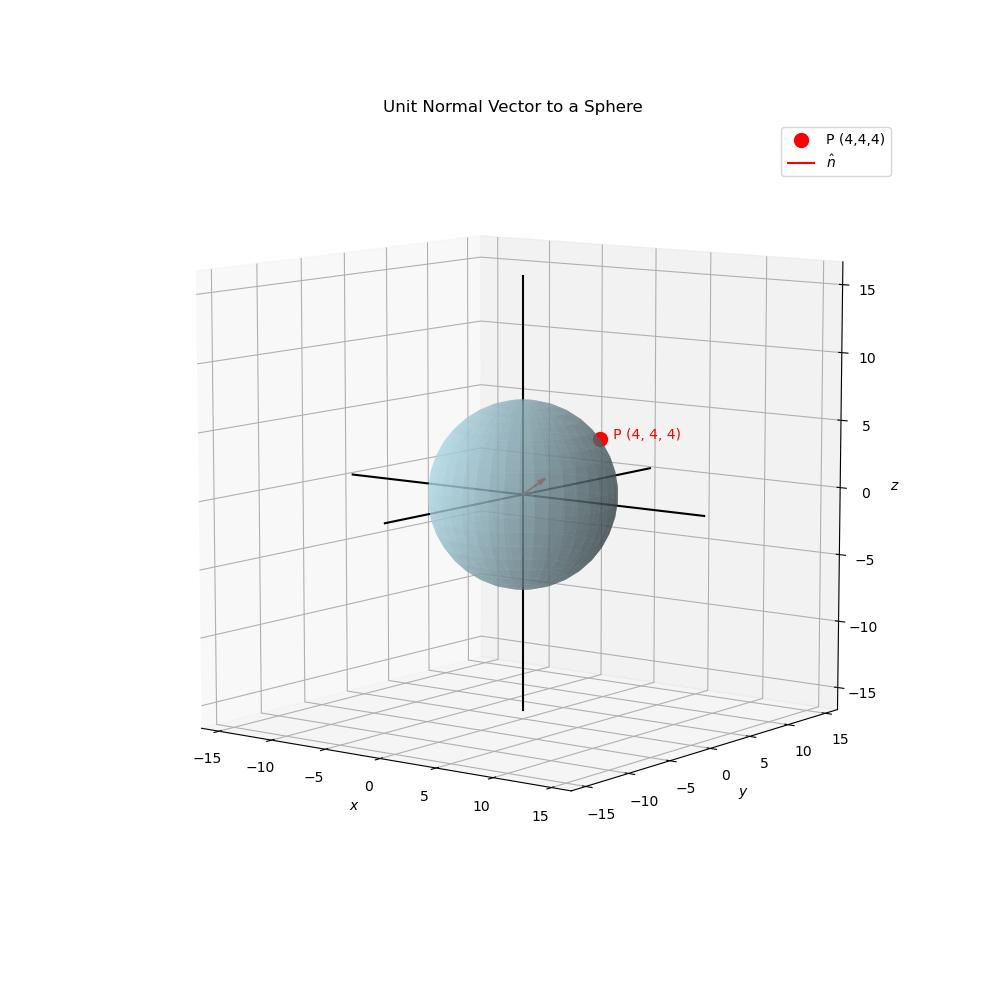
\includegraphics[width=\columnwidth]{figs/plot_c.jpg}
	\caption*{Plot}
	\label{fig:fig}
\end{figure}

\end{document}
